\documentclass[11pt]{article}
\usepackage{notes-common}

% Complete / filled-in reference version of gauss-applications-notes.tex (the
% PHYS 235 skeleton students fill in by hand). Same section structure and
% wording, but every diagram is drawn in and every blank carries the answer.
% Not meant to be handed out before class -- post it after, as a reference.
%
% Scope note: \derivbox areas are left as blank scratch space here too (they
% are genuinely "work it out" space, not a single-answer blank), except that
% each \result box now shows the final answer. Checkpoints get a short model
% answer instead of blank lines.

\newcommand{\ANS}[1]{\textcolor{accent}{#1}}

\begin{document}

\noteshead{More Gauss's Law --- the Three Symmetries \textcolor{accent}{(completed)}}{PHYS 235 \quad$\cdot$\quad Wed Sep 23 \quad$\cdot$\quad Knight 24.4--24.6}

\goal{State Gauss's law and understand what it says, then use it to \emph{compute}
$\vec{E}$ --- not just check it --- for the distributions where symmetry makes that
possible: a point charge and a shell, an infinite line, an infinite sheet, and a
uniformly charged sphere.}

%============================================================
\nsec{What Gauss's law says}

\textbf{a) Flux.} The number of electric field lines that exit or enter a
\ANS{closed surface} is the same, no matter the \ANS{size or shape} of the surface. By
``number of field lines'' we mean \emph{flux}:
\[
\Phi = {}\ANS{\oint \vec{E}\cdot d\vec{A}}
\]
Notes: the surface's area vector is \ANS{perpendicular} to the surface and points
\ANS{outward}, by convention. If lines are exiting, $\Phi$ is \ANS{positive}; if entering,
$\Phi$ is \ANS{negative}. A line that just passes through counts $+1$ for leaving and
$-1$ for entering, so it contributes \ANS{zero} net.

\textbf{b) Relation to charge.} The number of field lines --- also called \ANS{net flux}
--- through a closed surface is equal to \ANS{$q_{\text{enc}}/\varepsilon_0$}. Does it
matter how far from the charge the surface is? \ANS{No.} The closed surface we integrate
over is called a \ANS{Gaussian surface}.

\checkpoint{A point charge sits at the center of a Gaussian sphere. If you double the
sphere's radius, does $\Phi$ change? Does $E$ at the surface change? (Different questions!)}
{\small\color{accent} $\Phi$ doesn't change (same enclosed charge). $E$ \emph{does} change
--- it drops by a factor of 4, since $E=q/(4\pi\varepsilon_0 r^2)$ even though the total
flux through the bigger sphere is the same.}

%============================================================
\nsec{Using it: match the surface to the symmetry}

\textbf{a)} Use Gauss's law when the charge distribution has one of the three classical
symmetries: \ANS{spherical}, \ANS{cylindrical}, \ANS{planar}.

\textit{Definition of symmetry:} \ANS{If you closed your eyes while the charge
distribution changed in a symmetric way, then opened them again, you couldn't tell
anything had changed.}

\textbf{b)} Choose a Gaussian surface that respects the \ANS{symmetry} of the charge
distribution. If the distribution is spherically symmetric, make your surface spherically
symmetric too, \ANS{centered on the charge distribution} (similarly for cylindrical and
planar symmetry).

If you've done this, $\vec E$ will be everywhere either \ANS{parallel} or
\ANS{perpendicular} to your Gaussian surface, and will have the same \ANS{magnitude}
at every point on the surface, and $\Phi=E\oint dA=EA$ --- Gauss's law
becomes plain algebra: $EA=q_{\text{enc}}/\varepsilon_0$.

\checkpoint{Why does a cube fail as a Gaussian surface for a single point charge?}
{\small\color{accent} On a cube's faces $\vec E$ is neither constant in magnitude nor
everywhere parallel/perpendicular to the face --- both the distance to the charge and the
angle between $\vec E$ and $d\vec A$ vary across each face, so $E$ can't be pulled out of
the integral.}

\newpage
%============================================================
\nsec{Warm-up: a point charge, then a shell}

\begin{center}
\begin{tikzpicture}[x=0.85cm,y=0.85cm]
  \filldraw[red!70!black] (0,0) circle (0.09);
  \node[red!70!black, scale=0.9] at (-0.4,-0.05) {$+q$};
  \draw[gray!55, dashed] (0,0) circle (1.7);
  \foreach \a in {20,65,110,155,200,250,295,340}{
    \draw[cyan!65!black, ->, line width=0.8pt] (\a:0.25) -- (\a:1.7);}
  \draw[gray, ->] (0,0) -- (40:1.7);
  \node[scale=0.9, accent] at (40:2.15) {$r$};
\end{tikzpicture}
\end{center}

By symmetry $\vec E$ is radial and constant in magnitude on the sphere, so
$EA=q_{\text{enc}}/\varepsilon_0$ with $A=4\pi r^2$ and $q_{\text{enc}}=q$ gives
$E={}$\ANS{$\dfrac{1}{4\pi\varepsilon_0}\dfrac{q}{r^2}$} --- Coulomb's law, recovered from
Gauss's law.

Now make it a thin \textbf{shell} of charge $Q$, radius $R$, instead of a point.
\textbf{Outside} ($r>R$): the Gaussian sphere encloses \ANS{$Q$ (all of it)}, so
$E={}$\ANS{$\dfrac{1}{4\pi\varepsilon_0}\dfrac{Q}{r^2}$} (identical to a point charge ---
the shell might as well not have a size). \textbf{Inside} ($r<R$): the Gaussian sphere
encloses \ANS{$0$}, so $E={}$\ANS{$0$}.

\checkpoint{The sphere you'll work below is \emph{solid}, not a shell --- charge fills
the whole volume. Will its field inside behave the same way as the shell's?}
{\small\color{accent} No --- a solid sphere DOES enclose charge inside radius $r$ (it grows
with $r^3$), so unlike the shell, $E\neq0$ inside. See the result below: $E\propto r$.}

%============================================================
\nsec{Infinite line of charge}

Linear charge density $\lambda$. $\vec{E}$ points radially out from the wire and cannot
depend on position along it, so the Gaussian surface is a \emph{coaxial cylinder} of
radius $r$ and length $L$.

\begin{center}
\begin{tikzpicture}[x=0.88cm,y=0.88cm]
  \draw[red!70!black, line width=1.1pt] (0,-2.0) -- (0,2.0);
  \node[red!70!black, scale=0.8] at (0,2.25) {$\infty$};
  \node[red!70!black, scale=0.8] at (0,-2.25) {$\infty$};
  \draw[gray!55, dashed] (-1.4,1.05) -- (-1.4,-1.05);
  \draw[gray!55, dashed] (1.4,1.05) -- (1.4,-1.05);
  \draw[gray!55, dashed] (0,1.05) ellipse (1.4 and 0.38);
  \draw[gray!55, dashed] (0,-1.05) ellipse (1.4 and 0.38);
  \foreach \y in {-0.45,0.45}{
    \draw[cyan!65!black, ->, line width=0.9pt] (0.12,\y) -- (2.05,\y);
    \draw[cyan!65!black, ->, line width=0.9pt] (-0.12,\y) -- (-2.05,\y);
  }
  \node[scale=0.9, accent] at (2.95,0.45) {$\vec E$};
  \draw[gray, <->] (0,1.05) -- (1.4,1.05);
  \node[scale=0.9, accent] at (0.7,1.45) {$r$};
  \draw[gray, <->] (-2.6,-1.05) -- (-2.6,1.05);
  \node[scale=0.9, accent] at (-3.5,0) {$L$};
  \draw[gray!70, ->] (-3.0,-1.9) -- (-3.0,-1.35) node[above, scale=0.7] {$z$};
  \draw[gray!70, ->] (-3.0,-1.9) -- (-3.4,-2.25) node[below left, scale=0.7] {$x$};
  \draw[gray!70, ->] (-3.0,-1.9) -- (-2.55,-2.15) node[below right, scale=0.7] {$y$};
\end{tikzpicture}
\end{center}

\derivbox{2.2cm}{Which part of the cylinder carries flux (and which carries none)? Area $A$, then $q_{\text{enc}}$, then solve for $E$. Show $L$ cancelling.}

\ANS{Only the curved side carries flux ($\vec E\parallel d\vec A$ there); the flat end
caps carry none ($\vec E\perp d\vec A$). $A_{\text{side}}=2\pi rL$, $q_{\text{enc}}=\lambda
L$, so $E(2\pi rL)=\lambda L/\varepsilon_0$ --- $L$ cancels.}

\result{$E$ for an infinite line \quad\ANS{$E=\dfrac{\lambda}{2\pi\varepsilon_0 r}$}}

%============================================================
\nsec{Infinite sheet of charge}

Surface charge density $\eta$. This is a \emph{plane}, not a line: it extends forever in
\emph{two} directions, $x$ and $y$, and $\vec{E}$ points straight away from it along $\pm z$
on both sides.

\begin{center}
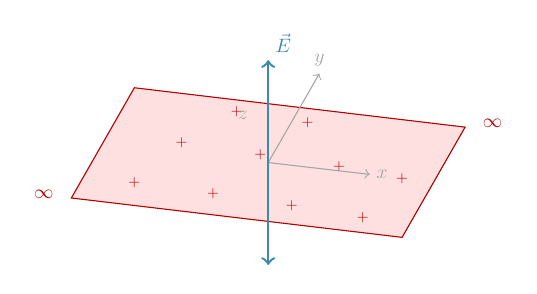
\begin{tikzpicture}[x=1cm,y=1cm]
  \fill[red!12] (-2.4,-0.4) -- (1.8,-0.9) -- (2.6,0.5) -- (-1.6,1.0) -- cycle;
  \draw[red!70!black] (-2.4,-0.4) -- (1.8,-0.9) -- (2.6,0.5) -- (-1.6,1.0) -- cycle;
  \foreach \p in {(-1.6,-0.2),(-0.6,-0.35),(0.4,-0.5),(1.3,-0.65),
                  (-1.0,0.3),(0.0,0.15),(1.0,0.0),(1.8,-0.15),
                  (-0.3,0.7),(0.6,0.55)}{
    \node[red!70!black, scale=0.55] at \p {$+$};}
  \node[red!70!black, scale=0.7] at (-2.75,-0.35) {$\infty$};
  \node[red!70!black, scale=0.7] at (2.95,0.55) {$\infty$};
  \coordinate (O) at (0.1,0.05);
  \draw[gray!70, ->] (O) -- ++(1.29,-0.15) node[right, scale=0.7] {$x$};
  \draw[gray!70, ->] (O) -- ++(0.65,1.13) node[above, scale=0.7] {$y$};
  \draw[cyan!65!black, ->, line width=0.9pt] (O) -- ++(0,1.3) node[above right, scale=0.7, cyan!65!black] {$\vec E$};
  \node[gray!70, scale=0.7] at (-0.22,0.65) {$z$};
  \draw[cyan!65!black, ->, line width=0.9pt] (O) -- ++(0,-1.3);
\end{tikzpicture}
\end{center}
\figtask{An infinite sheet, seen at an angle: it extends forever in $x$ \emph{and} $y$,
and $\vec E$ points straight out along $z$ on either side.}

Now look at it \emph{edge-on} (sighting along $y$, so the sheet appears as a line and the
pillbox is easy to draw), with end caps of area $A_{\text{cap}}$:

\begin{center}
\begin{tikzpicture}[x=0.9cm,y=0.9cm]
  \draw[red!70!black, line width=0.8pt] (-3.1,0) -- (3.1,0);
  \foreach \x in {-2.7,-1.8,-0.9,0,0.9,1.8,2.7}{
    \node[red!70!black, scale=0.62] at (\x,0.24) {$+$};}
  \node[red!70!black, scale=0.8] at (-3.4,0) {$\infty$};
  \node[red!70!black, scale=0.8] at (3.4,0) {$\infty$};
  \draw[gray!55, dashed] (-1.15,-0.9) rectangle (1.15,0.9);
  \draw[gray!55, dashed] (0,0.9) ellipse (1.15 and 0.28);
  \draw[gray!55, dashed] (0,-0.9) ellipse (1.15 and 0.28);
  \foreach \x in {-0.5,0.5}{
    \draw[cyan!65!black, ->, line width=0.9pt] (\x,0.95) -- (\x,1.95);
    \draw[cyan!65!black, ->, line width=0.9pt] (\x,-0.95) -- (\x,-1.95);
  }
  \node[scale=0.9, accent] at (2.0,1.75) {$\vec E$};
  \draw[gray, <->] (-1.6,-0.9) -- (-1.6,0);
  \node[scale=0.9, accent] at (-2.7,-0.45) {$h$};
  \draw[gray, <->] (-1.15,-2.35) -- (1.15,-2.35);
  \node[scale=0.9, accent] at (0,-2.75) {$A_{\text{cap}}$};
\end{tikzpicture}
\end{center}

\derivbox{2.0cm}{Total area carrying flux, $q_{\text{enc}}$ in terms of $\eta$ and $A_{\text{cap}}$, then $E$.}

\ANS{Both caps carry flux, total area $2A_{\text{cap}}$; $q_{\text{enc}}=\eta
A_{\text{cap}}$; so $E(2A_{\text{cap}})=\eta A_{\text{cap}}/\varepsilon_0$ --- $A_{\text{cap}}$
cancels.}

\result{$E$ for an infinite sheet \quad\ANS{$E=\dfrac{\eta}{2\varepsilon_0}$}}

\checkpoint{Two surprises. $A_{\text{cap}}$ cancelled --- why did it \emph{have} to? And the
answer contains no $r$ at all. What does that say about walking away from the sheet?}
{\small\color{accent} $A_{\text{cap}}$ had to cancel because both $\Phi$ and $q_{\text{enc}}$
scale with it equally --- $E$ can't depend on the size of a Gaussian surface you chose
arbitrarily. No $r$: the field is the \emph{same} at any distance --- the sheet looks
``infinite'' from any distance you could walk to.}

\textbf{Then: two parallel sheets}, one $+\eta$ and one $-\eta$. Superpose the two fields
you just found --- nothing new to derive.

\begin{center}
\begin{tikzpicture}[x=0.9cm,y=0.9cm]
  \draw[red!70!black, line width=0.8pt] (-2.6,0.9) -- (2.6,0.9);
  \foreach \x in {-2.2,-1.4,-0.6,0.2,1.0,1.8}{
    \node[red!70!black, scale=0.62] at (\x,1.14) {$+$};}
  \draw[blue!60!black, line width=0.8pt] (-2.6,-0.9) -- (2.6,-0.9);
  \foreach \x in {-2.2,-1.4,-0.6,0.2,1.0,1.8}{
    \node[blue!60!black, scale=0.62] at (\x,-1.14) {$-$};}
  \node[scale=0.85, accent] at (0,0) {$E=\eta/\varepsilon_0$};
  \node[scale=0.85, accent] at (0,1.95) {$E=0$};
  \node[scale=0.85, accent] at (0,-1.95) {$E=0$};
\end{tikzpicture}
\end{center}

%============================================================
\nsec{Uniformly charged sphere}

Total charge $Q$ spread uniformly through a solid sphere of radius $R$. There are two
regions, and the only difference between them is $q_{\text{enc}}$.

\begin{center}
\begin{tikzpicture}[x=0.8cm,y=0.8cm]
  \fill[red!16] (0,0) circle (1.1);
  \draw[red!70!black] (0,0) circle (1.1);
  \draw[gray!55, dashed] (0,0) circle (1.95);
  \foreach \a in {70,110,150,190,230,270,310}{
    \draw[cyan!65!black, ->, line width=0.8pt] (\a:1.95) -- (\a:2.6);}
  \draw[gray, ->] (0,0) -- (18:1.1);
  \node[scale=0.9, accent] at (2.15,0.42) {$R$};
  \draw[gray, dotted] (18:1.1) -- (1.7,0.42);
  \draw[gray, ->] (0,0) -- (-20:1.95);
  \node[scale=0.9, accent] at (2.75,-0.72) {$r$};
  \draw[gray, dotted] (-20:1.95) -- (2.3,-0.72);
\end{tikzpicture}
\end{center}

\textbf{Outside} ($r > R$): the Gaussian sphere encloses \ANS{all $Q$} of the charge.

\derivbox{1.6cm}{$q_{\text{enc}}$, then $E$. What familiar result does this match?}

\ANS{$q_{\text{enc}}=Q$, so $E=\dfrac{1}{4\pi\varepsilon_0}\dfrac{Q}{r^2}$ --- matches a
point charge (and the shell above).}

\result[1.3cm]{$E$ outside the sphere \quad\ANS{$E=\dfrac{1}{4\pi\varepsilon_0}\dfrac{Q}{r^2}$}}

\textbf{Inside} ($r < R$): only the charge within radius $r$ counts. The charge fills the
\ANS{volume}, so the fraction enclosed is the ratio of \ANS{volumes, $r^3/R^3$}.

\derivbox{1.6cm}{$q_{\text{enc}} = {}$?\quad then $E = {}$?}

\ANS{$q_{\text{enc}}=Q(r/R)^3$, so $E=\dfrac{1}{4\pi\varepsilon_0}\dfrac{Qr}{R^3}$ ---
linear in $r$.}

\result[1.3cm]{$E$ inside the sphere \quad\ANS{$E=\dfrac{1}{4\pi\varepsilon_0}\dfrac{Qr}{R^3}$}}

\checkpoint{Sketch $E$ against $r$ across both regions. At $r=R$ --- jump, kink, or neither?}
{\small\color{accent} Neither a jump nor a gap --- $E$ is continuous at $r=R$ (both
formulas agree there). But there IS a kink: the slope changes from linear ($E\propto r$)
to falling ($E\propto1/r^2$).}

\begin{center}
\begin{tikzpicture}[x=1cm,y=1cm]
  \draw[gray!70, ->] (0,0) -- (7.6,0) node[right, scale=0.8] {$r$};
  \draw[gray!70, ->] (0,0) -- (0,1.9) node[above, scale=0.8] {$E$};
  \draw[gray!35, dashed] (2.5,0) -- (2.5,1.75);
  \node[gray, scale=0.8] at (2.5,-0.32) {$R$};
  \draw[accent, line width=1pt] (0,0) -- (2.5,1.75);
  \draw[accent, line width=1pt, domain=2.5:7.3, samples=40]
    plot (\x, {1.75*(2.5/\x)^2});
\end{tikzpicture}
\end{center}

{\small\color{blankink} All three results are in the \emph{Applying Gauss's Law} sim ---
open its \textbf{Info} panel to check yours.}

\end{document}
